%%%%%%%%%%%%%%%%%%%%%%%%%%%%%%%%%%%%%%%%%%%%%%%%%%%%%%%%%%%%%%%%%%%%%%%%%%%%%%%%%%%%%%%%%%%%%
%											IMPLEMENTATION AND MEASUREMENTS																				%
%%%%%%%%%%%%%%%%%%%%%%%%%%%%%%%%%%%%%%%%%%%%%%%%%%%%%%%%%%%%%%%%%%%%%%%%%%%%%%%%%%%%%%%%%%%%%
\chapter{EXPERIMENTAL RESULTS}
\label{sec:experiments}
This chapter analyses the performances of the advanced model-based computed-torque controller. The experiments are conducted in the system that has the following configuration

\begin{flushleft}
Operating system - Ubuntu 14.04 LTS 64-bit \\
Processor - I5-7$^{th}$ generation
\end{flushleft}

\section{Model-based controller}

Torque controller is tested in youBot base at first to verify the logic of the controller before it is tested in the manipulator where the joint constraints are applicable. At first, the experiments are conducted for the safety controller interface to make sure that the safety layer is functioning properly or not in case of a logical error in the controller. The initial configuration of manipulator is assumed to be in candle as same as the 3-D model provided by the manufacturer, then the torque is commanded to the joint where the artificial position, velocity, torque limits are applied which is then replaced with the actual joint limits with a threshold of 0.5 rad in both the maximum and minimum limits of the manipulator joints. The threshold is introduced to avoid hitting the limits of the joints if the set-point is located near the joint limits. The artificial joint limits for the position, velocity, torque are 1.0 rad, 0.5 rad/s, 1.0 N.m. respectively. Once the joint limits are reached, the safety layer gets active and stops the controller to avoid any damages to the manipulator since the prolonged motion even after the breach in the safety limits could damage the system. The same experiments are conducted with the actual joint limits and the safety controller interface is breaking in the right place where the safety limits are breached. The real concern of the safety controller in high-speed motions is that the joint crosses the safety limit before the safety check is performed. The cause of this problem is that the controller is functioning in a non real-time system. 

\begin{table}[H]
\centering
\begin{tabular}{|c|c|l|l|}
\hline
\multirow{2}{*}{\textbf{PI Controller}} & \multicolumn{1}{l|}{\multirow{2}{*}{\textbf{Gains}}} & \multicolumn{2}{l|}{\textbf{Joint No.}}                           \\ \cline{3-4} 
                                        & \multicolumn{1}{l|}{}                                & \multicolumn{1}{c|}{\textbf{4}} & \multicolumn{1}{c|}{\textbf{5}} \\ \hline
\multirow{2}{*}{\textbf{Position}}      & P                                                    & 0.820                           & 1.900                           \\ \cline{2-4} 
                                        & I                                                    & 0.063                           & 0.033                           \\ \hline
\multirow{2}{*}{\textbf{Velocity}}      & P                                                    & 2.900                           & 1.500                           \\ \cline{2-4} 
                                        & I                                                    & 0.180                           & 0.120                           \\ \hline
\end{tabular}
\caption{Controller gains for the joints 4,5 after the empirical tuning procedure}
\end{table}

Basic approach is experimented prior to the alternate approach. The model-based controller based on the basic approach is successfully achieving the gravity compensation in the youBot manipulator that is based on KDL ID solver and the cascaded PI controller is also tested in the youBot manipulator. The main observation from this experiment is that the control variable $\ddot{q}$ computed by the cascaded controller is fed as an acceleration input to the KDL based solver where the model torques are generated which results in a very minimal torque ($10^{-5} N.m.$). These model torques were not sufficient enough to move the joints of the manipulator to the desired configuration. The reason behind this problem is that the inertial parameters are not accurate and rotor inertia should also be considered rather than just considering the links' moments of inertia. The static friction compensation is also experimented to move the joint from the equilibrium state and the identified static friction values from the previous work~\cite{RnD2Rajagopal} were not sufficient to move the joint from the rest state. So, the static friction value for the joints are increased to overcome the static friction on the manipulator joints. Once the joint started moving, the Coulomb friction torques were added with the model torques that compensates the dynamic friction. The alternate method that is used in this work is not having the friction compensation with it due to the fact that the model does only two things such as the gravity compensation and accounting the bias forces. Since the cascaded controller is implemented in this work, it is important to tune both the position and velocity controller gains to the optimum, empirically. The inner-loop and outer-loop controller has been tested with the different velocity set-points to check whether the tuned parameters are optimum or not. The empirical tuning of the controller gains for both the inner-loop and outer-loop with the velocity of 0.5 rad/s are depicted in the Figures~\ref{fig:innerloop_tuning0pt5rads}~\ref{fig:outerloop_tuning0pt5rads} respectively for the joint number 5. Since the measured velocity from the encoders are quite noisy as it is shown in Fig.~\ref{fig:innerloop_tuning0pt5rads}, the measured data is smoothed with the moving average filter that filters the noise with the window size 10. The smoothed data is helpful in understanding whether the set-point in the inner-loop has reached or not. The steady-state error with the threshold of 0.02 rad/s are assumed to be accepted in the inner-loop when tuning the controller gains due to the presence of noise but the ultimate goal of this project is to achieve the zero steady-state error. The outer-loop tuning is quite straight-forward where the joint  position set-point 0.5 rad is commanded to the joint and the result of the movement confirms the optimality of the controller gains. The additional tuning experiments with the different position and velocity set-points for the joint 5 can be found in the appendix~\ref{sec:appendixD}. 

\begin{figure}[H]
\centering     %%% not \center
\subfigure[Inner loop tuning]{\label{fig:innerloop_tuning0pt5rads}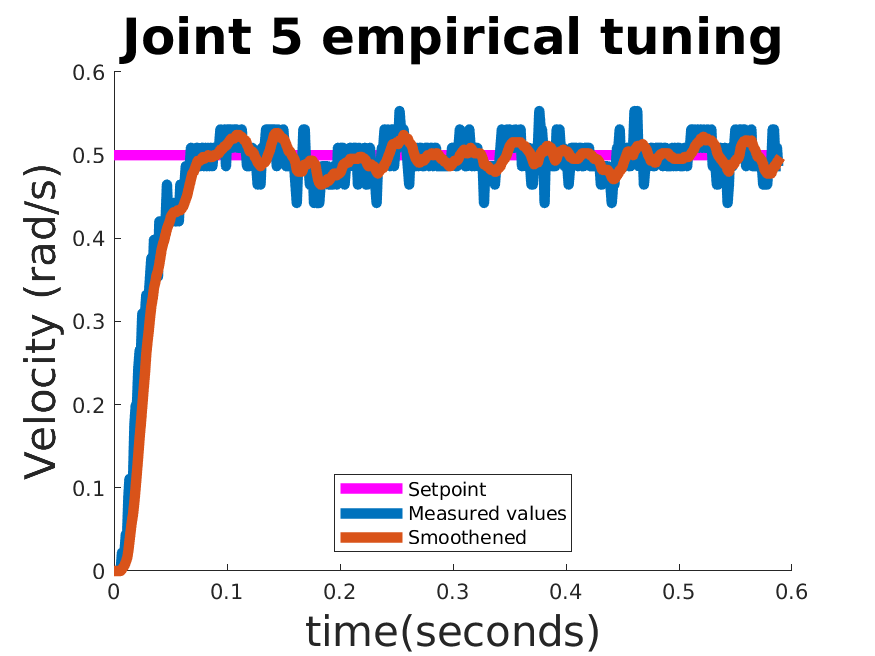
\includegraphics[width=70mm]{pictures/joint5_innerloop_0pt5rads}}
\subfigure[Outerloop tuning]{\label{fig:outerloop_tuning0pt5rads}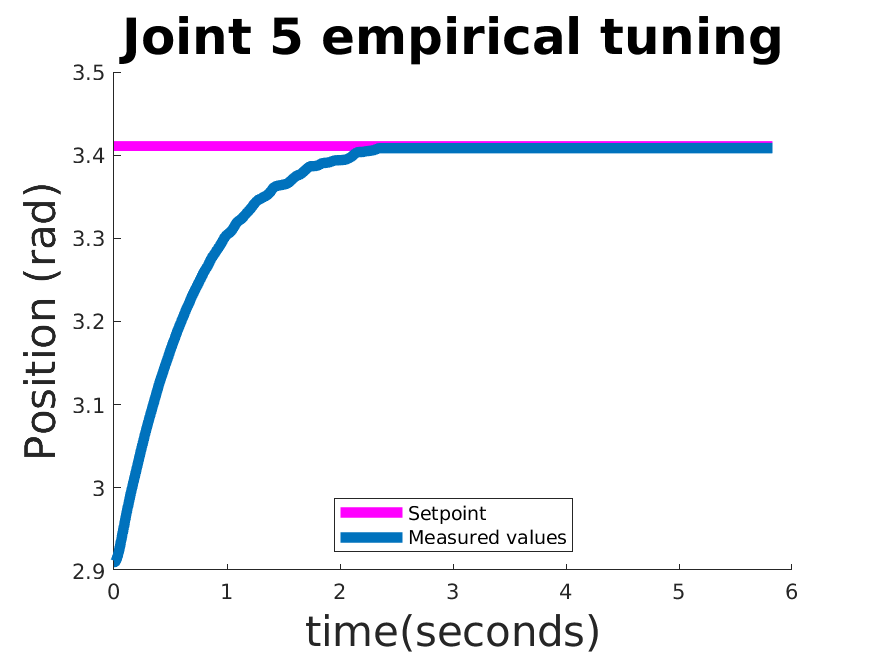
\includegraphics[width=70mm]{pictures/joint5_outerloop_0pt5rad}}
\caption{Inner, outer loop tuning for joint 5 with the velocity, position set-points of 0.5 rad/s, 0.5 rad respectively}
\end{figure}

After the controller gains are tuned to optimal values based on the set-points and the controller response, the individual joints of the manipulator can be evaluated with the analytical sine wave form as depicted in Fig.~\ref{fig:trajectorytrackingjoint5} since the computed-torque controller is attached in the joint level. The way-points of the sine waveform are generated in accordance with the controller frequency. In each and every cycle of the controller, a new position set-point (the way-points of the sine waveform) is commanded and the response is observed for the purpose of evaluation. 

\begin{figure}[H]
\centering
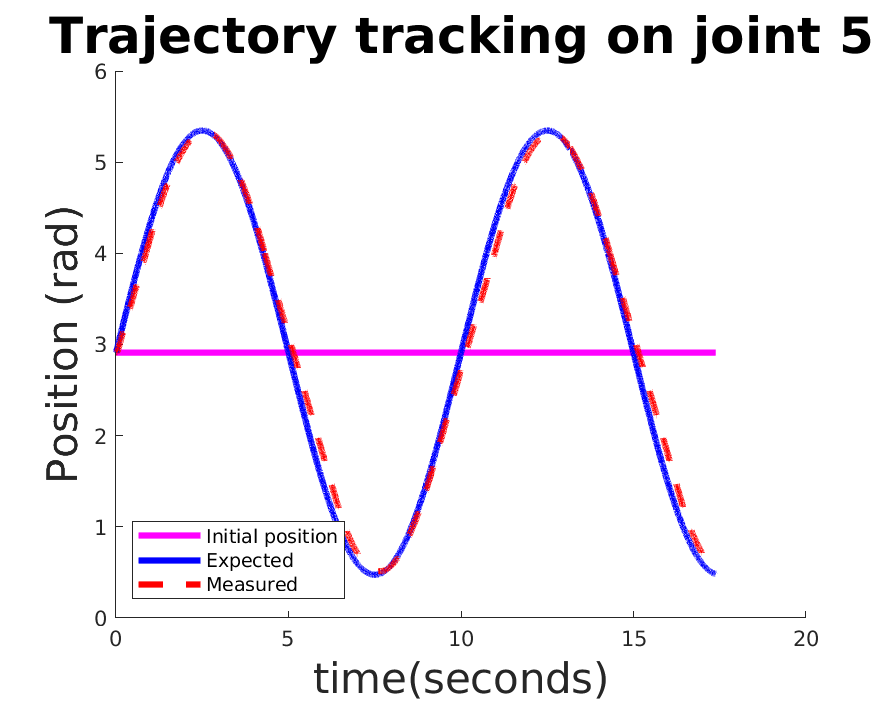
\includegraphics[width=90mm, trim=0 20 0 20]{pictures/joint5_trajectory}
\caption{Trajectory tracking experiment using the sine wave on joint 5}
\label{fig:trajectorytrackingjoint5}
\end{figure}

The error between the set-point and the controller response for all the way-points of the sine wave are depicted in Fig.~\ref{fig:trajectorytrackingerrorjoint5}. The maximum error that has been observed in joint number 5 is 0.3171 rad at some point in time. 

\begin{figure}[H]
\centering
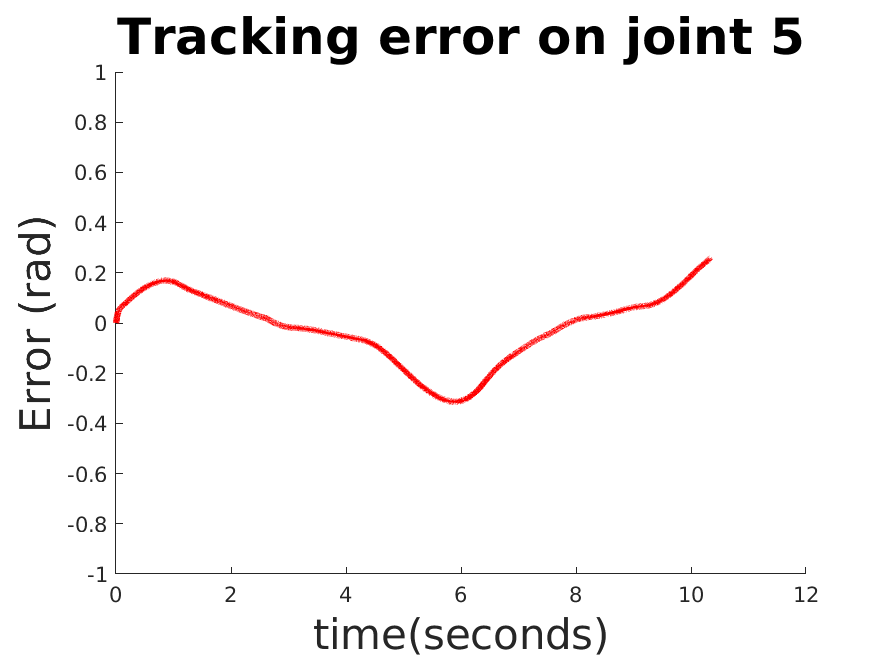
\includegraphics[width=90mm, trim=0 20 0 20]{pictures/joint5_trajectoryerror}
\caption{Trajectory tracking error on joint 5}
\label{fig:trajectorytrackingerrorjoint5}
\end{figure}

The controller gains are tuned for the joint 4 as depicted in the Figures~\ref{fig:innerloop_tuning0pt5rads_joint4}~\ref{fig:outerloop_tuning0pt5rads_joint4} which follows the same procedure that has been followed for the joint number 5. 

\begin{figure}[H]
\centering     %%% not \center
\subfigure[Inner loop tuning]{\label{fig:innerloop_tuning0pt5rads_joint4}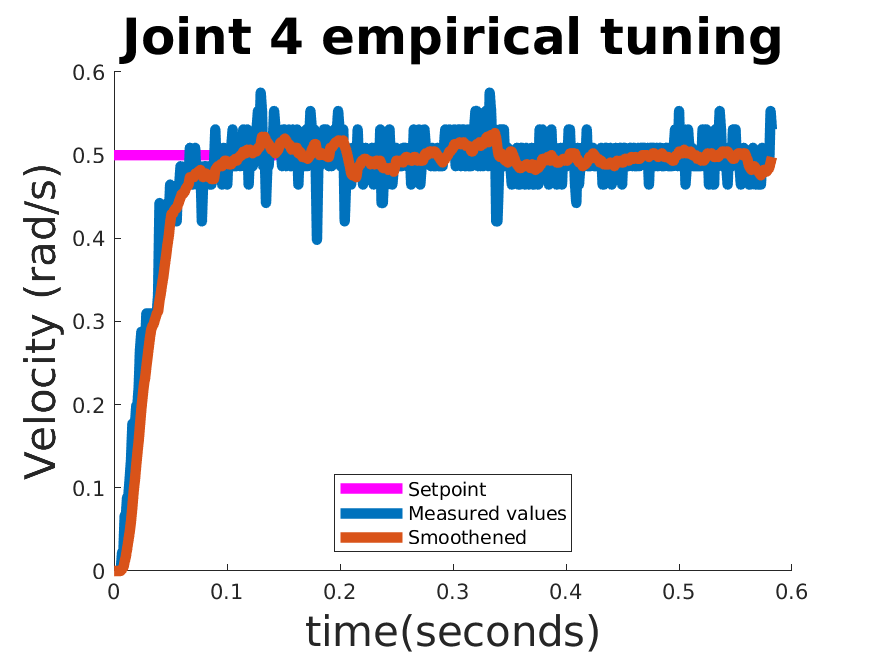
\includegraphics[width=70mm]{pictures/joint4_innerloop_0pt5rads}}
\subfigure[Outerloop tuning]{\label{fig:outerloop_tuning0pt5rads_joint4}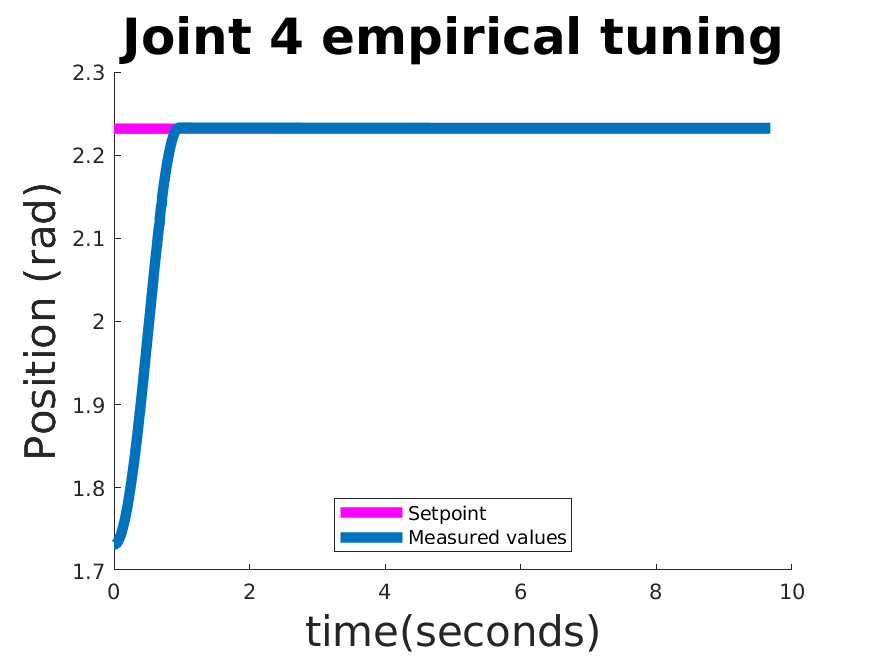
\includegraphics[width=70mm]{pictures/joint4_outerloop_0pt5rad}}
\caption{Inner, outer loop tuning for joint 4 with the velocity, position set-points of 0.5 rad/s, 0.5 rad respectively}
\end{figure}

\begin{figure}[H]
\centering
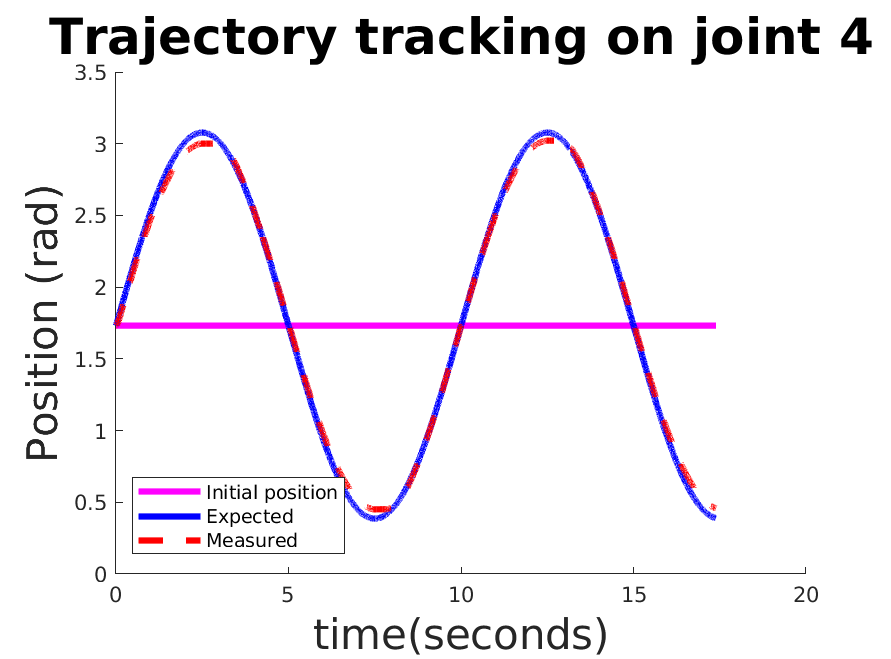
\includegraphics[width=90mm, trim=0 20 0 20]{pictures/joint4_trajectory}
\caption{Trajectory tracking experiment using the sine wave on joint 4}
\label{fig:trajectorytrackingjoint4}
\end{figure}

The error between the set-point and the controller response for all the way-points of the sine wave are depicted in Fig.~\ref{fig:trajectorytrackingerrorjoint4}. The maximum error that has been observed in joint number 4 is 0.0779 rad at some point in time. 

\begin{figure}[H]
\centering
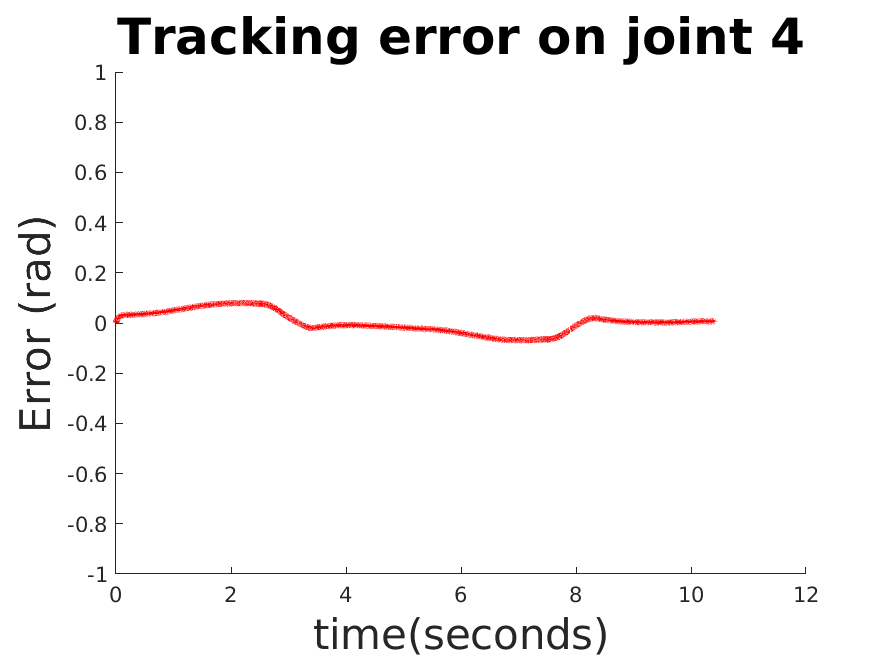
\includegraphics[width=90mm, trim=0 20 0 20]{pictures/joint4_trajectoryerror}
\caption{Trajectory tracking error on joint 4}
\label{fig:trajectorytrackingerrorjoint4}
\end{figure}

The trajectory tracking error is caused due to many reasons such as the controller gains are not be optimal yet hence the tuning has to be re-considered, the presence of the cascaded controller where the optimality of the inner-loop control gains are suffering due to the noise in the measured data. The following Fig.~\ref{fig:ratiojoint4} depicts the model, controller torques w.r.t. the position of joint 4.

\begin{figure}[H]
\centering
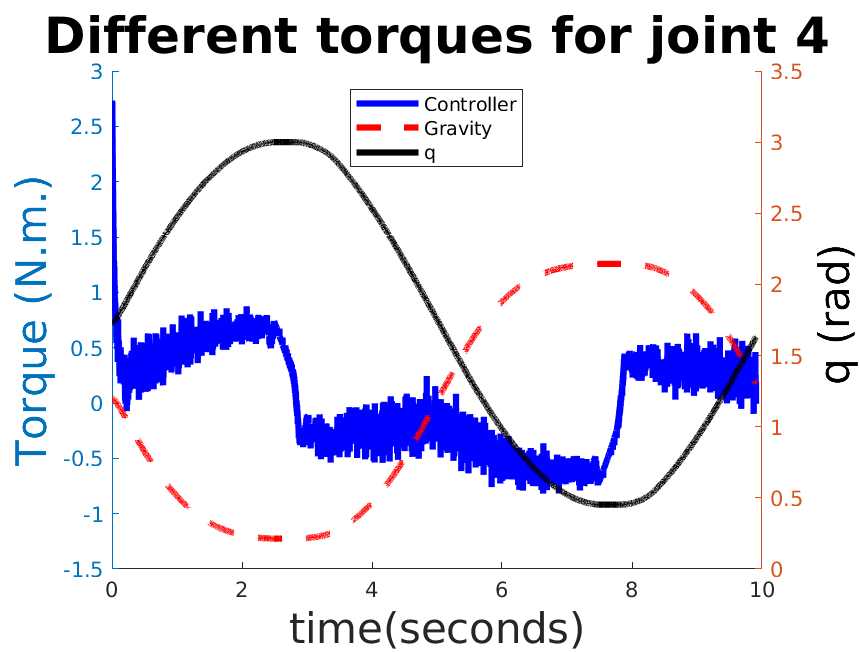
\includegraphics[width=90mm, trim=0 0 0 0]{pictures/joint4_ratio}
\caption{Modeled torque and controller torques are shown w.r.t. time along with the angular position for joint 4}
\label{fig:ratiojoint4}
\end{figure}

It can be clearly seen that torque generated by the model do not have high frequency noise as expected. Again, the controller handles the disturbances in the manipulator joints producing high-frequency components. An important cause of this problem is that the model discrepancies introduce deviations in torque prediction which in-turn has a huge impact on the advanced model based controller. The friction compensation terms in the dynamic model would improve the controller's performance further. Though the dynamic model is incomplete, the controller is able to follow the trajectories close-enough with a minimal deviations. The non real-time system is used for the development that produces latency issues in the feedback-control system. 

\section{Inertial parameter estimation}

The inertial model parameters provided by the manufacturers are inaccurate and the identification of the model parameters are not complete. It is decided to go with the mass and CoM where the rotational inertia parameters are ignored in the system model of the youBot manipulator. The link parameters without the rotational inertia has been tested on the real robot for the gravity compensation and the joints are not sliding due to gravitational pull hence the link properties of the dynamic model in Orocos KDL excludes the rotational inertia in the computations.